\section{Durchführung}
\label{sec:Durchführung}

Das Experiment zur Bestimmung der Wärmeleitfähigkeit ist in Abb. \ref{fig:versuch} dargestellt. 
Auf einer Grundplatte liegen vier Proben aus drei verschiedenen Materialien. 
Die vier Stäbe werden von einem Peltierelement geheizt und gekühlt.
Ein Peltierelement besteht aus Halbleitern und basiert auf dem Peltier-Effekt.
Es erzeugt bei Stromdurchfluss eine Temperaturdifferenz.
Die Temperaturen werden an zwei Stellen an jedem Stab mit 
Thermoelementen gemessen und an einen Datenlogger weitergegeben.
\begin{figure}
    \centering
    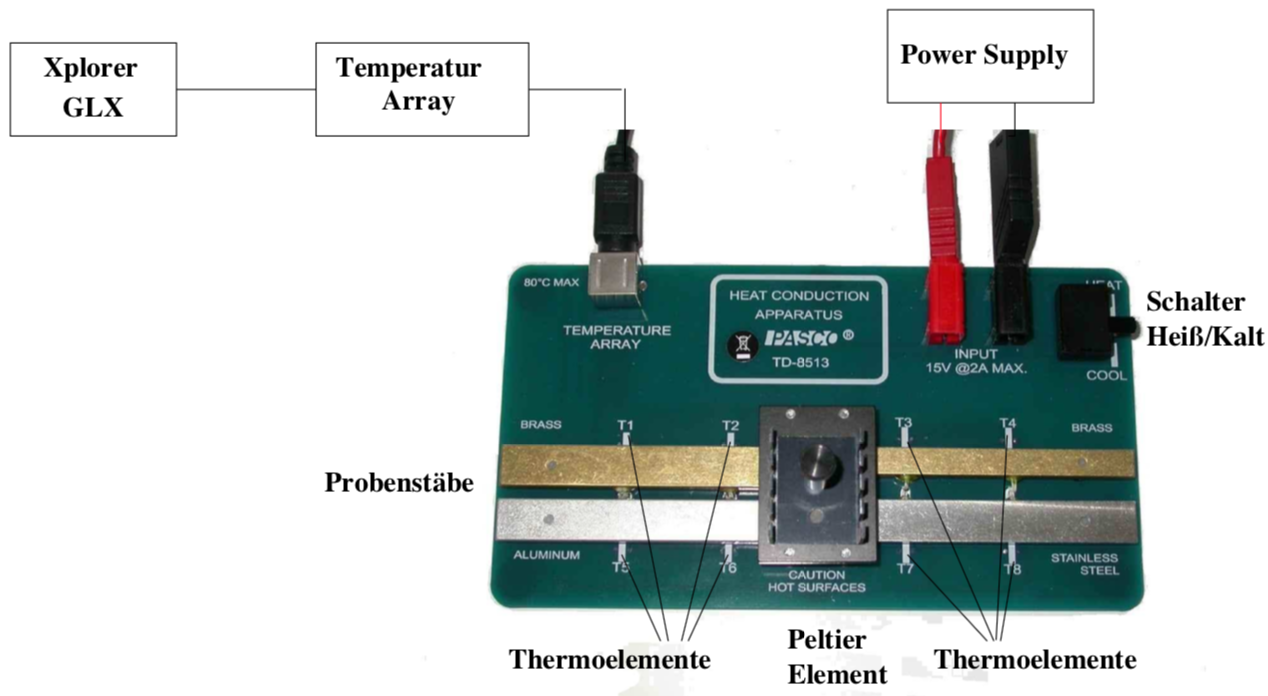
\includegraphics[scale=0.2]{build/aufbau.png}
    \caption{Versuchsaufbau.}
    \label{fig:versuch}
\end{figure}

\noindent Zwischen den Messungen werden die Stäbe wieder auf unter $\SI{30}{\degreeCelsius}$ abgekühlt

\subsection{Statische Methode}
Zunächst wird der zeitliche Verlauf der Temperatur der Stäbe 
mit der statischen Methode untersucht.
Dafür werden die Stäbe $\SI{700}{\second}$ lang erhitzt.
Dabei werden jeweils Werte im Abstand von $\SI{5}{\second}$ aufgenommen.
Der Verlauf für die Thermoelemente
$T1$, $T4$, $T5$ und $T8$ wird graphisch dargestellt und ausgedruckt.
Dies sind die fernen Thermoelemente.
Die Verläufe der Differenzen der Thermoelemente des Edelstahlstabes $\Delta T = T7 - T8$
und der des breiten Messingstabes $\Delta T = T2 - T1$ werden ebenfalls graphisch dargestellt und
ausgedruckt.
Außerdem werden $\num{5}$ Temperaturen in einem Abstand von $\SI{140}{\second}$
für die vier fernen Thermoelemente gemessen.
Die jeweiligen Abstände der nahen und der fernen Thermoelemente werden gemessen.

\subsection{Dynamische Methode für Messing und Aluminium}
Die Stäbe werden nun periodische erhitzt bzw. gekühlt.
Die Werte werden in einem Abstand von $\SI{2}{\second}$ aufgenommen.
Eine Periode beträgt $\SI{80}{\second}$. Die Stäbe werden also jeweils
$\SI{40}{\second}$ lang erhitzt und anschließend $\SI{40}{\second}$
lang gekühlt.
Es werden $\num{10}$ Perioden
gemessen. %oder hatten wir 11?
Die Temperaturverläufe für Messing (Thermoelemente $T1$ und $T2$)
und für Aluminium (Thermoelemente $T5$ und $T6$)
werden graphisch dargestellt und ausgedruckt.

\subsection{Dynamische Methode für Edelstahl}
Eine Periode beträgt $\SI{200}{\second}$.
Die Stäbe werden also $\SI{100}{\second}$ lang erhitzt und anschließend 
$\SI{100}{\second}$ lang gekühlt.
Es werden $\num{11.5}$ Perioden gemessen.
%bzw. so lange, bis ein Thermoelement $\SI{80}{\degreeCelsius}$ erreicht.
Die Temperaturverläufe des Edelstahlstabes (Thermoelemente $T7$ und $T8$)
werden graphisch dargestellt und ausgedruckt.